% Journals and co\begin{document}
\section{Publications}\label{publications}
{\large
In 2013 we published 50 internationally reviewed papers, more than any year before in the history of CBA, see Figure~\ref{fig:publications}. There are several reasons for this, but the main one is that after two years without PhD dissertations there will be about eight new CBA doctors in 2014 and PhD students publish most at the end of their studies. Another reason is that we have more researcher than before and are involved in more co-operation projects. 

In our research field the quality and impact of many conference proceedings are higher than many of the Journals. As the proceedings also usually are a faster way to publish we often chose that outlet of our results. But of course we also publish in scientific journals, especially when reporting results on medical applications in co-operation with medical researchers, as that field is more journal oriented. 

This year we edited the proceedings of the ISMM conference which was published in the prestigious Springer Lecture notes in Computer Science. We published 29 journal articles in journals as different as the theoretical Computer Vision and Image Understanding and prestigious Nature Methods, from Artificial Intelligence Tools to Magnetic Resonance Imaging and Composite Science and Technology. We also published 21 papers in fully reviewed conference proceedings; both at meetings dedicated to the theory of image analysis, such as DGCI, ISMM, and SIGGRAPH, and to more application oriented ones, such as HIP, ISBI, and WHC. We also had many presentations at non-reviewed conferences. 

%
%FROM LAST YEAR 
%We consider the publication of our results very important and a measure of the quality of our work. Hence, all research projects we are involved in (see Section~\ref{research}) should result in one or more publications. 
%Most often we publish in international scientific journals and fully refereed international conference proceedings; this is true for work both on theory and on different applications.
%
%In our research field, the impact factor of some of the conferences is higher than well-reputed journals, so in some cases we prefer to submit high-quality work to a conference rather than to a journal. 
%In order to meet other scientists, we sometimes publish in
%non-reviewed conferences, but those results are usually eventually also published elsewhere. We aim to produce some popular science articles, but are less successful in this respect. However, we do give a number of such seminars each year.
%
%
%This list covers all publications with publication date in 2013.
%%We have published chapters in two books.
%%We have edited one conference proceedings. 
%UPDATE THE TEXT
%We have published 14~journal articles and 20~articles in fully-reviewed international conference proceedings.
%In addition, we published 14 papers in workshops, non-refereed or abstract refereed conference proceedings, and three other reports. The number of fully reviewed publications from CBA between 2001--2012 is shown in Figure~\ref{fig:publications}.% These numbers indicate a very productive year for CBA. 
%
\begin{figure}[!h] 
\centering
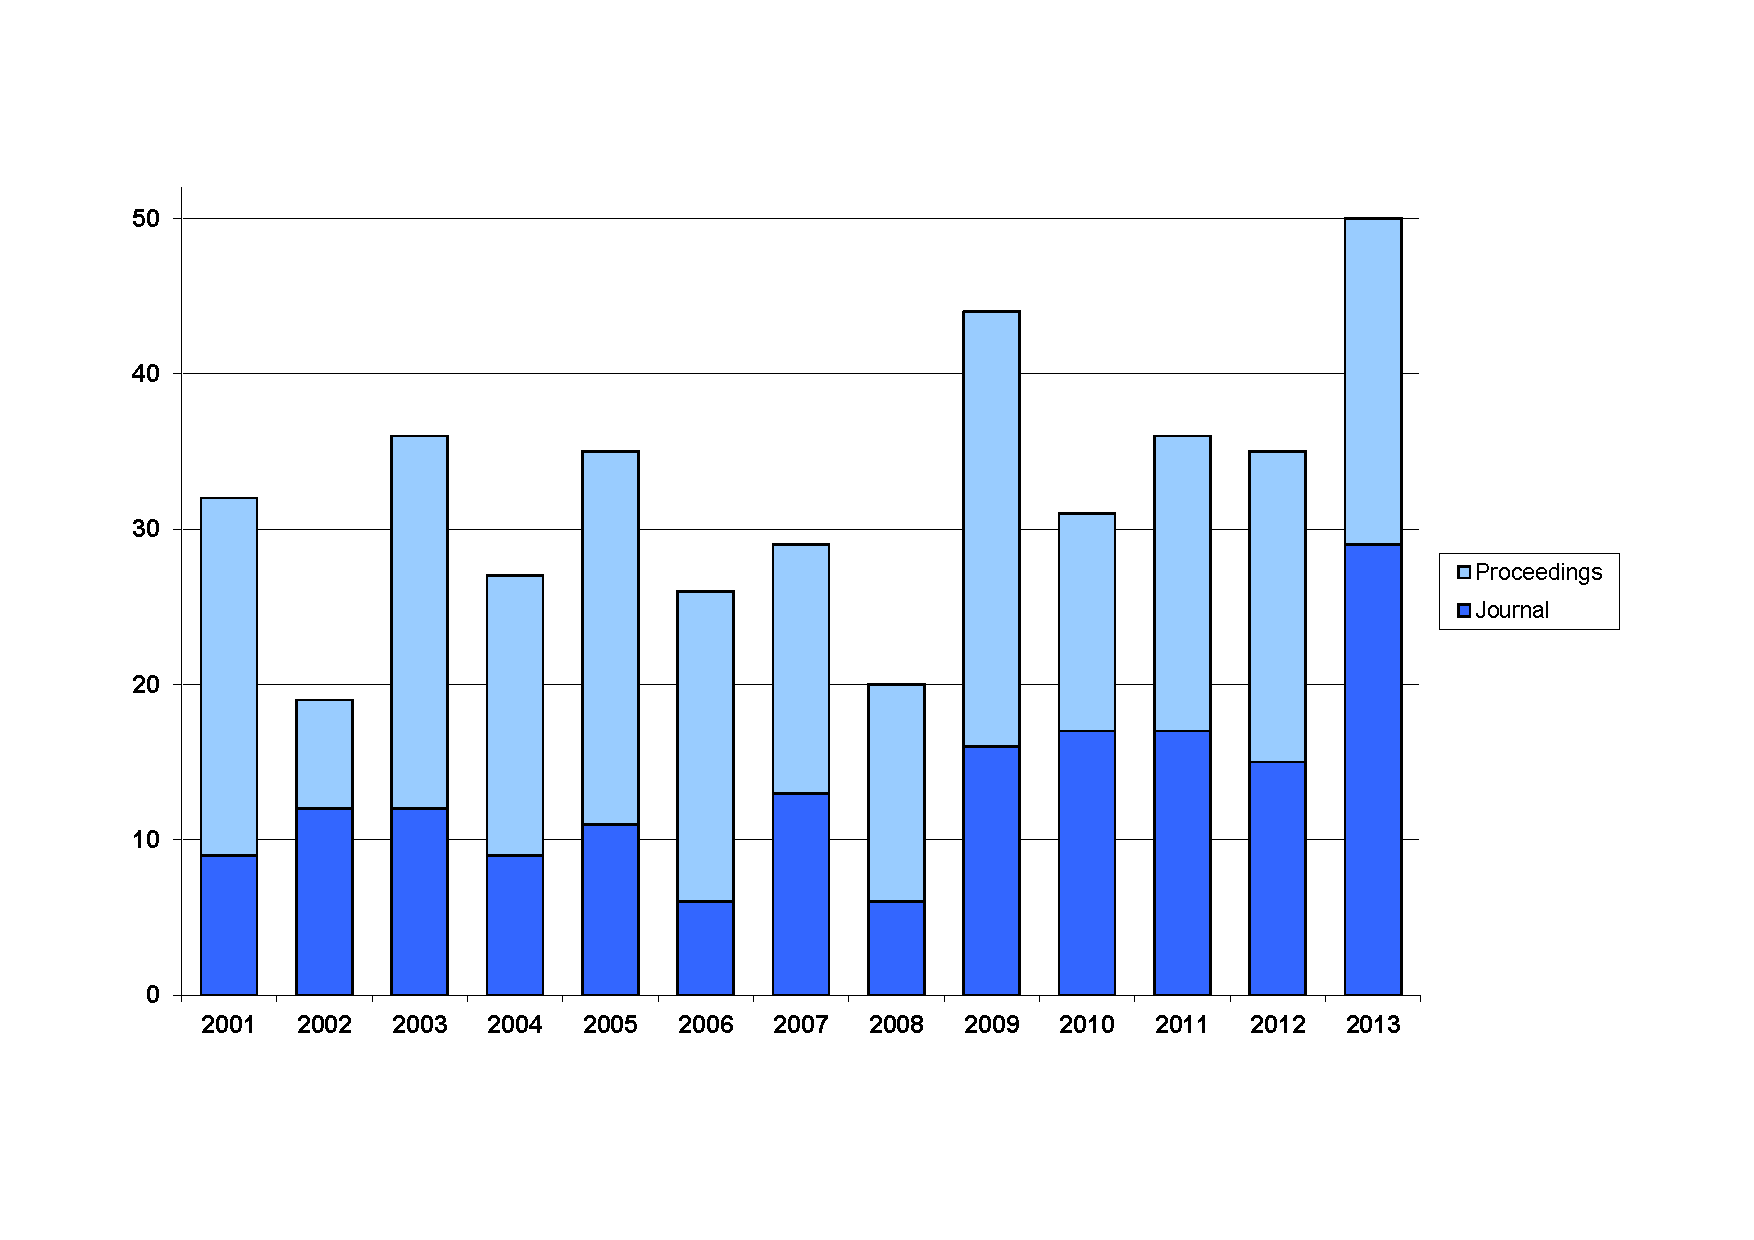
\includegraphics[angle=0, width=0.8\textwidth, viewport=50 100 790 520, clip]{./figures/CBA_pub_2013.pdf}
\caption{The number of publications from CBA.
\label{fig:publications}}
\end{figure}
}

%\subsection{Patents}\label{sect:patent}
%{\small
%\begin{enumerate}
%\ttitle{Patent title }
%{\em Inventors:} \\
%{\em Pub. No.:} \\
%{\em Pub. Date.:} \\
%{\em Abstract:} 
%\end{enumerate}
%}


%\newpage
%\subsection{Book chapters}\label{sect:book}
%
%{\small 
%
%\begin{enumerate}
%
%\ttitle{Structural Characterisation of Kraft Pulp Fibres and Their Nanofibrillated Materials for Biodegradable Composite Applications}
%\aauthors{Gary Chinga-Carrasco (1), Arttu Miettinen (2), {\bf Cris L. Luengo Hendriks}, E. Kristofer Gamstedt (3), and Markku Kataja (2)\\
%(1) Paper and Fibre Research Institute (PFI), Norway\\
%(2) Dept.~of Physics, University of Jyv\"{a}skyl\"{a}, Finland\\
%(3) Uppsala University, Disciplinary Domain of Science and Technology, Technology, Dept.~of Engineering Sciences, Applied Mechanics
%}
%\bbook{Nanocomposites and Polymers with Analytical Methods, pp 243-260}
%\eeditor{John Cuppoletti}
%\ppublisher{InTech, Rijeka, Croatia}
%
%\ttitle{Rapid Prototyping of Image Analysis Applications}
%\aauthors{{\bf Cris L. Luengo Hendriks}, {\bf Patrik Malm}, and {\bf Ewert Bengtsson}}
%\bbook{Medical Image Processing: Techniques and Applications, Biological and Medical Physics, Biomedical Engineering Series, pp 5-25}
%\eeditor{Geoff Dougherty}
%\ppublisher{Springer, New York}
%\end{enumerate}
%}%small
%
%\newpage
\subsection{Edited conference proceedings}
Editors affiliated with CBA are written in bold.
%%
{\small

\begin{enumerate}
%BibTex
\item
\textbf{Conference name:} 11th International Symposium on Mathematical Morphology and Its Applications to Signal and Image Processing\\
\emph{Editors:} {\bf Cris L.~Luengo Hendriks, Gunilla Borgefors, Robin Strand}\\
\emph{Comment:} The conference was held in Uppsala in May. The proceedings is Lecture Notes in Computer Science, No. 7883, Springer Verlag, 532 pages.

%@proceedings{659551,
% editor = {Luengo Hendriks, Cris L. and Borgefors, Gunilla and Strand, Robin},
% institution = {Uppsala University, Division of Visual Information and Interaction},
% institution = {Uppsala University, Computerized Image Analysis and Human-Computer Interaction},
% pages = {532},
% title = {Mathematical Morphology and Its Applications to Signal and Image Processing : 11th International Symposium, ISMM 2013; Uppsala, Sweden, May 2013; Proceedings},
% series = {Lecture Notes in Computer Science},
% number = {7883},
% year = {2013}
%}

%%\item X
%%%
%%\item
%%\textbf{Conference name:} Interaction in Medical Image Analysis and Visualization\\
%%\emph{Editors:\/} Smedby, .(1); Bengtsson, E.; Persson, A.(1)\\
%%(1) Center for Medical Image Science and Visualization (CMIV), Linkping University\\
%%\emph{Comment:\/} Workshop at 10th International Conference on Medical Image Computing and Computer Assisted Intervention (MICCAI 2007), Brisbane, Australia, 2007. 96 pages.
%%
%
%
\end{enumerate}
%%}

%\clearpage
\subsection{Journal articles}\label{sect:journal}
% always Abstract when existing
%
\vspace*{-0.3mm}
Authors affiliated with CBA are in bold.
{\small
\vspace*{-0.5mm}
\begin{enumerate}
\ttitle{Improving the Stochastic Watershed}
\aauthors{{\bf Karl B. Bernander, Kenneth Gustavsson, Bettina Selig, Ida-Maria Sintorn, Cris L. Luengo Hendriks}}
\jjournal{Pattern Recognition Letters, volume 34, number 9, pages 993-1000}
\\ \aabstract
The stochastic watershed is an unsupervised segmentation tool recently proposed by Angulo and Jeulin. By repeated application of the seeded watershed with randomly placed markers, a probability density function for object boundaries is created. In a second step, the algorithm then generates a meaningful segmentation of the image using this probability density function. The method performs best when the image contains regions of similar size, since it tends to break up larger regions and merge smaller ones. We propose two simple modifications that greatly improve the properties of the stochastic watershed: (1) add noise to the input image at every iteration, and (2) distribute the markers using a randomly placed grid. The noise strength is a new parameter to be set, but the output of the algorithm is not very sensitive to this value. In return, the output becomes less sensitive to the two parameters of the standard algorithm. The improved algorithm does not break up larger regions, effectively making the algorithm useful for a larger class of segmentation problems.


\ttitle{A Fast and Reliable Approach to Cell Nuclei Segmentation in PAP Stained Cervical Smears}
\aauthors{Balakrishnan Bujy (1), Vilayil Sujathan (2) {\bf Patrik Malm}, Rajesh Kumar (1)\\ 
(1) CDAC Thiruvananthapuram, India\\
(2) Regional Cancer Centre, Thiruvananthapuram, India}
\jjournal{CSI Transactions on ICT, Volume 1, number 4, pages 309-315}
\\ \aabstract
Fast and reliable segmentation of cervical cell nuclei is one of the crucial steps of an automated screening system that aims early detection of cervical cancer. In this paper, we propose an edge based approach using customized Laplacian of Gaussian (LoG) filter to segment free lying cell nuclei in bright-field microscope images of Papsmear. The LoG is generally employed as a second order edge detector in image processing. The images may have the challenges of inconsistent staining, overlapping and folded cells. Experimenting proposed method over all types of cervical images including sufficient number of high grade lesions of cervical cancer shows that our method performs well for stain varied images containing focused nuclei.


\ttitle{Virtual Surgery "Virtuell Kirurgi"}
\aauthor{{\bf Ingrid Carlbom}, Mats Karlsson}
\jjournal{Tandl\"{a}kartidningen, number 6, pages 12-15}
\\ \aabstract
Virtual surgery - a dream? Not at all; in just a few years it might be the reality. The surgeon can already today perform a virtual rehearsal of the real surgery. (in Swedish)
 
%Virtuell operation - en utopi? Inte alls; om bara n{\aa}gra {\aa}r kan det vara verklighet. Kirurgen kan redan f\"{o}re den verkliga operationen genomf\"{o}ra ett genrep virtuellt.

\ttitle{Blind Color Decomposition of Histological Images}
\aauthors {{\bf Milan Gavrilovic, Jimmy Azar}, {\bf Joakim Lindblad}, {\bf Carolina W{\"a}hlby}, {\bf Ewert Bengtsson}, Christer Busch (1), {\bf Ingrid Carlbom}\\
(1) Dept.~of Immunology, Genetics and Pathology, Uppsala University}
\jjournal{IEEE Transactions on Medical Imaging, volume 32, number 6, pages 983-994}
\\ \aabstract
Cancer diagnosis is based on visual examination under a microscope of tissue sections from biopsies. But whereas pathologists rely on tissue stains to identify morphological features, automated tissue recognition using color is fraught with problems that stem from image intensity variations due to variations in tissue preparation, variations in spectral signatures of the stained tissue, spectral overlap and spatial aliasing in acquisition, and noise at image acquisition. We present a blind method for color decomposition of histological images. The method decouples intensity from color information and bases the decomposition only on the tissue absorption characteristics of each stain. By modeling the charge-coupled device sensor noise, we improve the method accuracy. We extend current linear decomposition methods to include stained tissues where one spectral signature cannot be separated from all combinations of the other tissues' spectral signatures. We demonstrate both qualitatively and quantitatively that our method results in more accurate decompositions than methods based on non-negative matrix factorization and independent component analysis. The result is one density map for each stained tissue type that classifies portions of pixels into the correct stained tissue allowing accurate identification of morphological features that may be linked to cancer.
 

\ttitle {Canine Body Composition Quantification Using 3 Tesla Fat\- Water MRI}
\aauthors {Aliya Gifford (1), Joel Kullberg (1), Johan Berglund (1), {\bf Filip Malmberg}, Katie C. Coate (2), Phillip E. Williams (2), Alan D. Cherrington(2), Malcolm J. Avison(2), E. Brian Welch (2)\\
(1) Dept.~of Radiology, Uppsala University\\
(2)  Institute of Imaging Science,Vanderbilt University, Nashville, TN, USA}
\jjournal {Journal of Magnetic Resonance Imaging}
\\ \aabstract
Purpose: To test the hypothesis that a whole-body fat-water MRI (FWMRI) protocol acquired at 3 Tesla combined with semi-automated image analysis techniques enables precise volume and mass quantification of adipose, lean, and bone tissue depots that agree with static scale mass and scale mass changes in the context of a longitudinal study of large-breed dogs placed on an obesogenic high-fat, high-fructose diet.

Materials and methods: Six healthy adult male dogs were scanned twice, at weeks 0 (baseline) and 4, of the dietary regiment. FWMRI-derived volumes of adipose tissue (total, visceral, and subcutaneous), lean tissue, and cortical bone were quantified using a semi-automated approach. Volumes were converted to masses using published tissue densities.

Results: FWMRI-derived total mass corresponds with scale mass with a concordance correlation coefficient of 0.931 (95\% confidence interval $= [0.813, 0.975]$), and slope and intercept values of 1.12 and -2.23 kg, respectively. Visceral, subcutaneous and total adipose tissue masses increased significantly from weeks 0 to 4, while neither cortical bone nor lean tissue masses changed significantly. This is evidenced by a mean percent change of 70.2\% for visceral, 67.0\% for subcutaneous, and 67.1\% for total adipose tissue.

Conclusion: FWMRI can precisely quantify and map body composition with respect to adipose, lean, and bone tissue depots. The described approach provides a valuable tool to examine the role of distinct tissue depots in an established animal model of human metabolic disease."
 
 
\ttitle{Optimal RANSAC - Towards a Repeatable Algorithm for Finding the Optimal Set}
\aauthors{{\bf Anders Hast},  {\bf Johan Nysj{\"o}}}
\jjournal {Journal of WSCG, volume 21, number 1, pages 21-30}
\\ \aabstract
A novel idea on how to make RANSAC repeatable is presented, which will find the optimal set in nearly every run for certain types of applications. The proposed algorithm can be used for such transformations that can be constructed by more than the minimal points required. We give examples on matching of aerial images using the Direct Linear Transformation, which requires at least four points. Moreover, we give examples on how the algorithm can be used for finding a plane in 3D using three points or more. Due to its random nature, standard RANSAC is not always able to find the optimal set even for moderately contaminated sets and it usually performs badly when the number of inliers is less than 50\%. However, our algorithm is capable of finding the optimal set for heavily contaminated sets, even for an inlier ratio under 5\%. The proposed algorithm is based on several known methods, which we modify in a unique way and together they produce a result that is quite different from what each method can produce on its own.
%\newpage
\ttitle{Automated Classification of Immunostaining Patterns in Breast Tissue from the Human Protein Atlas}
\aauthors{Swamidoss Issac Niwas (1), {\bf Andreas K{\aa}rsn{\"a}s} (2), Virginie Uhlmann (3,4), P. Palanisamy (1), Caroline Kampf (4), {\bf Martin Simonsson} (5), {\bf Carolina W{\"a}hlby} (3,5), {\bf Robin Strand}\\
(1) Dept.~of Electronics and Communication Engineering (ECE), National Institute of Technology (NIT), Tiruchirappalli, India\\
(2) Visiopharm A/S, H{\o}rsholm, Denmark\\
(3) Imaging Platform, Broad Institute of Harvard and MIT, Cambridge, Massachusetts MA, USA\\ 
(4) Biomedical Imaging Group, \'{E}cole Polytechnique F\'{e}d\'{e}rale de Lausanne (EPFL), Switzerland\\
(5) Science for Life Laboratory, SciLifeLab, UU\\
(6) Dept.~Immunology, Genetics and Pathology, UU }
\jjournal {Journal of Pathology Informatics, volume 4, number 14}
\\ \aabstract
Background: The Human Protein Atlas (HPA) is an effort to map the location of all human proteins (http://www.proteinatlas.org/). It contains a large number of histological images of sections from human tissue. Tissue micro arrays (TMA) are imaged by a slide scanning microscope, and each image represents a thin slice of a tissue core with a dark brown antibody specific stain and a blue counter stain. When generating antibodies for protein profiling of the human proteome, an important step in the quality control is to compare staining patterns of different antibodies directed towards the same protein. This comparison is an ultimate control that the antibody recognizes the right protein. In this paper, we propose and evaluate different approaches for classifying sub-cellular antibody staining patterns in breast tissue samples. \\
Materials and Methods: The proposed methods include the computation of various features including gray level co-occurrence matrix (GLCM) features, complex wavelet co-occurrence matrix (CWCM) features, and weighted neighbor distance using compound hierarchy of algorithms representing morphology (WND-CHARM)-inspired features. The extracted features are used into two different multivariate classifiers (support vector machine (SVM) and linear discriminant analysis (LDA) classifier). Before extracting features, we use color deconvolution to separate different tissue components, such as the brownly stained positive regions and the blue cellular regions, in the immuno-stained TMA images of breast tissue. \\
Results: We present classification results based on combinations of feature measurements. The proposed complex wavelet features and the WND-CHARM features have accuracy similar to that of a human expert.\\
Conclusions: Both human experts and the proposed automated methods have difficulties discriminating between nuclear and cytoplasmic staining patterns. This is to a large extent due to mixed staining of nucleus and cytoplasm. Methods for quantification of staining patterns in histopathology have many applications, ranging from antibody quality control to tumor grading.
 
\ttitle{Color deconvolution method for breast tissue core biopsy images cell nuclei detection and analysis using multiresolution techniques}
\aauthors {Swamidoss Issac Niwas (1,2), P. Palanisamy (1), {\bf Ewert Bengtsson}\\
 (1) Dept.~of Electronics and Communication Engineering (ECE), National Institute of Technology (NIT), Tiruchirappalli, India\\
 (2) Science for Life Laboratory, SciLifeLab, UU}
\jjournal{International Journal of Imaging and Robotics, volume 9, number 1, pages 61-72}
\\ \aabstract
Breast cancer is the second most common cause of cancer induced death in women in the world. Testing for detection of the cancer involves visual microscopic assessment of breast tissue samples such as core needle biopsies. Analysis on this sample by pathologist is crucial for breast cancer patient. In this paper, a color deconvolution method is used to detect nuclei of core needle biopsy images and then it is investigated after decomposition by means of the curvelet transform. The curvelet statistical features are used for breast
 cancer diagnosis using the Naive Bayes Classifier (NBC) system. The ability of properly trained Naive Bayes Classifiers correctly classify and recognize patterns which is particularly suitable for use in an expert system assisting the diagnosis of cancer tissue samples.

\ttitle{Analysis of Nuclei Textures of Fine Needle Aspirated Cytology Images for Breast Cancer Diagnosis using Complex Daubechies Wavelets}
\aauthors{Swamidoss Issac Niwas (1,2), P. Palanisamy(1), K. Sujathan(3), {\bf Ewert Bengtsson}\\
(1) National Institute of Technology (NIT), Tiruchirappalli, India\\
(2) Science for Life Laboratory, SciLifeLab, UU\\
(3) Regional Cancer Centre, Thiruvanathapuram, India}
\jjournal{Signal Processing, volume 93, number 10, pages 2828-2837}
\\ \aabstract
Breast cancer is the most frequent cause of cancer induced death among women in the world. Diagnosis of this cancer can be done through radiological, surgical, and pathological assessments of breast tissue samples. A common test for detection of this cancer involves visual microscopic inspection of Fine Needle Aspiration Cytology (FNAC) samples of breast tissue. The result of analysis on this sample by a cytopathologist is crucial for the breast cancer patient. For the assessment of malignancy, the chromatin texture patterns of the cell nuclei are essential. Wavelet transforms have been shown to be good tools for extracting information about texture. In this paper, it has been investigated whether complex wavelets can provide better performance than the more common real valued wavelet transform. The features extracted through the wavelets are used as input to a k-nn classifier. The correct classification results are obtained as 93.9\% for the complex wavelets and 70.3\% for the real wavelets.

\ttitle {Swelling of Cellulose Fibres in Composite Materials : Constraint Effects of the Surrounding Matrix}
\aauthors{Thomas Joffre (1), {\bf Erik L. G. Wernersson}, Arttu Miettinen (2), {\bf Cris L. Luengo Hendriks}, E. Kristofer Gamstedt (1)\\
(1) Applied Materials Sciences, UU\\
(2) Dept.~Physiscs, University of Jyv{\"a}skyl{\"a}, Finland}
\jjournal {Composites Science And Technology, volume 74, pages 52-59}
\\ \aabstract
Wood fibres have several highly desirable properties as reinforcement in composite materials for structural applications, e.g. high specific stiffness and strength, renewability and low cost. However, one of the main drawbacks is the swelling of these hydrophilic fibres due to moisture uptake. Since the fibres in the composite are generally embedded in a relatively hydrophobic matrix, the surrounding matrix should restrain the swelling of the fibres. The present study investigates this constraint effect and establishes a micromechanical model to predict the swelling of embedded fibres based on experimentally characterised microstructural parameters and hygroelastic properties of the constituents. The predicted swelling is in concert with direct measurement of various wood-pulp fibre composites by means of three-dimensional X-ray microtomographic images.

\ttitle {In Situ Sequencing for RNA Analysis in Preserved Tissue and Cells}
\aauthors {Rongqin Ke (1,2), Marco Mignardi (1,2), {\bf Alexandra Pacureanu} (3), Jessica Svedlund (2), Johan Botling (1), {\bf Carolina W{\"a}hlby} (3,4), Mats Nilsson (1,2)\\
(1) Dept.~Immunology, Genetics and Pathology, UU\\
(2) Science for Life Laboratory, Department of Biochemistry and Biophysics, Stockholm University\\
(3) Science for Life Laboratory, SciLifeLab, UU\\
(4) Imaging Platform, Broad Institute of Harvard and Massachusetts Institute of Technology, Cambridge, Massachusetts, MA, USA}
\jjournal {Nature Methods, volume 10, number 9, pages 857-860}
\\ \aabstract
Tissue gene expression profiling is performed on homogenates or on populations of isolated single cells to resolve molecular states of different cell types. In both approaches, histological context is lost. We have developed an in situ sequencing method for parallel targeted analysis of short RNA fragments in morphologically preserved cells and tissue. We demonstrate in situ sequencing of point mutations and multiplexed gene expression profiling in human breast cancer tissue sections.

\ttitle {Shape and Volume of Craniofacial Cavities in Intentional Skull Deformations}
\aauthors {R.~H.~Khonsari~(1,2), M.~Friess~(3), {\bf Johan Nysj{\"o}}, G.~Odri~(4), {\bf Filip Malmberg}, {\bf Ingela Nystr{\"o}m}, Elias~Messo~(5), Jan~M.~Hirsch~(5), E.~A.~M.~Cabanis~(6), K.~H.~Kunzelmann~(7), J.~M.~Salagnac~(1), P.~Corre~(1), A.~Ohazama~(2), P.~T.~Sharpe~(2), P.~Charlier~(8), R.~Olszewski~(9)\\
(1) Service de Chirurgie Maxillofaciale et Stomatologie, CHU H\^{o}tel-Dieu, Nantes, France\\
(2) Department of Craniofacial Development and Stem Cell Research, Dental Institute, King's College London, UK\\
(3) D\'{e}partement Hommes, Natures, Soci\'{e}t\'{e}s \\ CNRS UMR 7206, Mus\'{e}um National d'Histoire Naturelle, Mus\'{e}e de l'Homme, Paris, France\\
(4) Clinique Chirurgicale Orthop\'{e}dique et Traumatologique, CHU H\^{o}tel-Dieu, Nantes, France\\
(5) Dept.~of Surgical Sciences, Oral and Maxillo-facial Surgery, Medical Faculty, UU\\
(6) Service de Neuroradiologie, Centre Hospitalier National Ophtalmologique des XV-XX, Paris, France\\
(7) Poliklinic f\"{u}r Zahnerhaltung und Parodontologie, Ludwig-Maximilians-Universit\"{a}t, M\"{u}nich, Germany\\
(8) Service d'anatomopathologie, H\^{o}pital Raymond-Poincar\'{e}, Garches, France\\
(9) Service de Chirurgie Maxillofaciale et Stomatologie, H\^{o}pital Saint-Luc, Universit\'{e} Catholique de Louvain, Bruxelles, Belgium}
\jjournal {American Journal of Physical Anthropology, volume 151, number 1, pages 110-119}
\\ \aabstract
Intentional cranial deformations (ICD) have been observed worldwide but are especially prevalent in preColombian cultures. The purpose of this study was to assess the consequences of ICD on three cranial cavities (intracranial cavity, orbits, and maxillary sinuses) and on cranial vault thickness, in order to screen for morphological changes due to the external constraints exerted by the deformation device. We acquired CT-scans for 39 deformed and 19 control skulls. We studied the thickness of the skull vault using qualitative and quantitative methods. We computed the volumes of the orbits, of the maxillary sinuses, and of the intracranial cavity using haptic-aided semi-automatic segmentation. We finally defined 3D distances and angles within orbits and maxillary sinuses based on 27 anatomical landmarks and measured these features on the 58 skulls. Our results show specific bone thickness patterns in some types of ICD, with localized thinning in regions subjected to increased pressure and thickening in other regions. Our findings confirm that volumes of the cranial cavities are not affected by ICDs but that the shapes of the orbits and of the maxillary sinuses are modified in circumferential deformations. We conclude that ICDs can modify the shape of the cranial cavities and the thickness of their walls but conserve their volumes. These results provide new insights into the morphological effects associated with ICDs and call for similar investigations in subjects with deformational plagiocephalies and craniosynostoses.

\ttitle{Evaluation of Noise Robustness for Local Binary Pattern Descriptors in Texture Classification}
\aauthors{{\bf Gustaf Kylberg}, {\bf Ida-Maria Sintorn}}
\jjournal{EURASIP Journal on Image and Video Processing, 2013:17, 20 pages}
\\ \aabstract
Local binary pattern (LBP) operators have become commonly used texture descriptors in recent years. Several new LBP-based descriptors have been proposed, of which some aim at improving robustness to noise. To do this, the thresholding and encoding schemes used in the descriptors are modified. In this article, the robustness to noise for the eight following LBP-based descriptors are evaluated; improved LBP, median binary patterns (MBP), local ternary patterns (LTP), improved LTP (ILTP), local quinary patterns, robust LBP, and fuzzy LBP (FLBP). To put their performance into perspective they are compared to three well-known reference descriptors; the classic LBP, Gabor filter banks (GF), and standard descriptors derived from gray-level co-occurrence matrices. In addition, a roughly five times faster implementation of the FLBP descriptor is presented, and a new descriptor which we call shift LBP is introduced as an even faster approximation to the FLBP. The texture descriptors are compared and evaluated on six texture datasets; Brodatz, KTH-TIPS2b, Kylberg, Mondial Marmi, UIUC, and a Virus texture dataset. After optimizing all parameters for each dataset the descriptors are evaluated under increasing levels of additive Gaussian white noise. The discriminating power of the texture descriptors is assessed using tenfolded cross-validation of a nearest neighbor classifier. The results show that several of the descriptors perform well at low levels of noise while they all suffer, to different degrees, from higher levels of introduced noise. In our tests, ILTP and FLBP show an overall good performance on several datasets. The GF are often very noise robust compared to the LBP-family under moderate to high levels of noise but not necessarily the best descriptor under low levels of added noise. In our tests, MBP is neither a good texture descriptor nor stable to noise.

\ttitle {Brain Pathology After Mild Traumatic Brain Injury: An Exploratory Study by Repeated Magnetic Resonance Examination}
\aauthors{Marianne Lannsj{\"o}~(1,2), Raili Raininko~(3), {\bf Mariana Bustamante (4)}, Charlotta von Seth~(1), J{\"o}rgen~Borg~(5)\\
(1) Dept.~Neuroscience, Rehabilitation Medicine, UU\\
(2) Centre for Research and Development, County Council of G\"{a}vleborg/UU\\
(3) Dept.~Radiology, UU\\
(4) M.Sc.~student, CBA\\
(5) Department of Clinical Sciences, Rehabilitation Medicine, Karolinska Institute, Danderyd Hospital, Stockholm}
\jjournal {Journal of Rehabilitation Medicine, volume 45, number 8, pages 721-728}
\\ \aabstract
Objective: To explore brain pathology after mild traumatic brain injury by repeated magnetic resonance examination.\\
Design: A prospective follow-up study.\\
Subjects: Nineteen patients with mild traumatic brain injury presenting with Glasgow Coma Scale (GCS) 14-15.\\
Methods: The patients were examined on day 2 or 3 and 3-7 months after the injury. The magnetic resonance protocol comprised conventional T1- and T2-weighted sequences including fluid attenuated inversion recovery (FLAIR), two susceptibility-weighted sequences to reveal haemorrhages, and diffusion-weighted sequences. Computer-aided volume comparison was performed. Clinical outcome was assessed by the Rivermead Post-Concussion Symptoms Questionnaire (RPQ), Hospital Anxiety and Depression Scale (HADS) and Glasgow Outcome Scale Extended (GOSE).\\
Results: At follow-up, 7 patients (37\%) reported $\geq 3$ symptoms in RPQ, 5 reported some anxiety and 1 reported mild depression. Fifteen patients reported upper level of good recovery and 4 patients lower level of good recovery (GOSE 8 and 7, respectively). Magnetic resonance pathology was found in 1 patient at the first examination, but 4 patients (21\%) showed volume loss at the second examination, at which 3 of them reported $< 3$ symptoms and 1 $\geq 3 $ symptoms, all exhibiting GOSE scores of 8.\\
Conclusion: Loss of brain volume, demonstrated by computer-aided magnetic resonance imaging volumetry, may be a feasible marker of brain pathology after mild traumatic brain injury.

\ttitle {Debris Removal in Pap-smear Images}  
\aauthors{{\bf Patrik Malm}, Byju N. Balakrishnan (1), Vilayil K. Sujathan (2), Rajesh Kumar (1), {\bf Ewert Bengtsson}\\
(1) Centre for Development of Advanced Computing, Thiruvananthapuram, India\\
(2) Regional Cancer Centre, Thiruvananthapuram, India}
\jjournal {Computer Methods and Programs in Biomedicine, volume 111, number 1, pages 128-138}
\\ \aabstract
Since its introduction in the 1940s the Pap-smear test has helped reduce the incidence of cervical cancer dramatically in countries where regular screening is standard. The automation of this procedure is an open problem that has been ongoing for over fifty years without reaching satisfactory results. Existing systems are discouragingly expensive and yet they are only able to make a correct distinction between normal and abnormal samples in a fraction of cases. Therefore, they are limited to acting as support for the cytotechnicians as they perform their manual screening. The main reason for the current limitations is that the automated systems struggle to overcome the complexity of the cell structures. Samples are covered in artefacts such as blood cells, overlapping and folded cells, and bacteria, that hamper the segmentation processes and generate large number of suspicious objects. The classifiers designed to differentiate between normal cells and pre-cancerous cells produce unpredictable results when classifying artefacts. In this paper, we propose a sequential classification scheme focused on removing unwanted objects, debris, from an initial segmentation result, intended to be run before the actual normal/abnormal classifier. The method has been evaluated using three separate datasets obtained from cervical samples prepared using both the standard Pap-smear approach as well as the more recent liquid based cytology sample preparation technique. We show success in removing more than 99\% of the debris without loosing more than around one percent of the epithelial cells detected by the segmentation process.

\ttitle {A New Algorithm for Computing Riemannian Geodesic Distance in Rectangular 2-D and 3-D Grids}
\aauthors {Ola Nilsson (1), Martin Reimers (2), Ken Museth (1), {\bf Anders Brun}\\
(1) Dept.~Science and Technology, Link\"{o}ping University\\
(2) Dept.~Informatics, University of Oslo, Norway}
\jjournal{International Journal on Artificial Intelligence Tools, volume 22, number 6, 25 pages}
\\ \aabstract
We present a novel way to efficiently compute Riemannian geodesic distance over a two- or three-dimensional domain. It is based on a previously presented method for computation of geodesic distances on surface meshes. Our method is adapted for rectangular grids, equipped with a variable anisotropic metric tensor. Processing and visualization of such tensor fields is common in certain applications, for instance structure tensor fields in image analysis and diffusion tensor fields in medical imaging.

The included benchmark study shows that our method provides significantly better results in anisotropic regions in 2-D and 3-D and is faster than current stat-of-the- art solvers in 2-D grids. Additionally, our method is straightforward to code; the test implementation is less than 150 lines of C++ code. The paper is an extension of a previously presented conference paper and includes new sections on 3-D grids in particular. 
 
\ttitle {Intracranial Volume Estimated with Commonly Used Methods Could Introduce Bias in Studies including Brain Volume Measurements}
\aauthors {Richard Nordenskj{\"o}ld (1), {\bf Filip Malmberg}, Elna-Marie Larsson (1), Andrew Simmons (2,3), Samatha J. Brooks (4), Lars Lind (5), H{\aa}kan Ahlstr{\"o}m (1), Lars Johansson (1,6), Joel Kullberg (1)\\
(1) Dept.~Radiology, UU\\
(2) King's College London, Institute of Psychiatry, London, UK\\
(3) NIHR Biomedical Research Centre for Mental Health and NIHR Biomedical Research Unit for Dementia, London, UK\\
(4) Dept.~Neuroscience, UU\\
(5) Dept.~Medical Sciences, UU\\
(6) AstraZeneca, M\"{o}lndal, Sweden}
\jjournal {NeuroImage, volume 83, pages 355-360}
\\ \aabstract
In brain volumetric studies, intracranial volume (ICV) is often used as an estimate of pre-morbid brain size as well as to compensate for inter-subject variations in head size. However, if the estimated ICV is biased by for example gender or atrophy, it could introduce errors in study results. To evaluate how two commonly used methods for ICV estimation perform, computer assisted reference segmentations were created and evaluated. Segmentations were created for 399 MRI volumes from 75-year-old subjects, with 53 of these subjects having an additional scan and segmentation created at age 80. ICV estimates from Statistical Parametric Mapping (SPM, version 8) and Freesurfer (FS, version 5.1.0) were compared to the reference segmentations, and bias related to skull size (approximated with the segmentation measure), gender or atrophy were tested for. The possible ICV related effect on associations between normalized hippocampal volume and factors gender, education and cognition was evaluated by normalizing hippocampal volume with different ICV measures. Excellent agreement was seen for inter- (r=0.999) and intra- (r=0.999) operator reference segmentations. Both SPM and FS overestimated ICV. SPM showed bias associated with gender and atrophy while FS showed bias dependent on skull size. All methods showed good correlation between time points in the longitudinal data (reference: 0.998, SPM: 0.962, FS: 0.995). Hippocampal volume showed different associations with cognition and gender depending on which ICV measure was used for hippocampal volume normalization. These results show that the choice of method used for ICV estimation can bias results in studies including brain volume measurements.

\ttitle {Minimal-Delay Distance Transform for Neighborhood-Sequence Distances in 2D and 3D}
\aauthors {Nicolas Normand (1), {\bf Robin Strand}, Pierre Evenou (1), Aurore Arlicot (1)\\
(1) Institut de Recherche en Communications et en Cybern\'{e}tique de Nantes (IRCCyN), France}
\jjournal {Computer Vision and Image Understanding, volume 117, number 4, pages 409-417}
\\ \aabstract
This paper presents a path-based distance, where local displacement costs vary both according to the displacement vector and with the travelled distance. The corresponding distance transform algorithm is similar in its form to classical propagation-based algorithms, but the more variable distance increments are either stored in look-up-tables or computed on-the-fly. These distances and distance transform extend neighborhood-sequence distances, chamfer distances and generalized distances based on Minkowski sums. We introduce algorithms to compute a translated version of a neighborhood sequence distance map both for periodic and aperiodic sequences and a method to derive the centered distance map. A decomposition of the grid neighbors, in $Z^2$ and $Z^3$, allows to significantly decrease the number of displacement vectors needed for the distance transform. Overall, the distance transform can be computed with minimal delay, without the need to wait for the whole input image before beginning to provide the result image

\ttitle {A Haptics-Assisted Cranio-Maxillofacial Surgery Planning System for Restoring Skeletal Anatomy in Complex Trauma Cases}
\aauthors {{\bf Pontus Olsson}, {\bf Fredrik Nysj{\"o}}, Jan-Micha{\'e}l Hirsch (1), {\bf Ingrid B. Carlbom}\\
(1) Dept.~Oral and Maxillofacial Surgery, UU}
\jjournal {International Journal of Computer Assisted Radiology and Surgery, volume 8, number 6, pages 887-894}
\\ \aabstract
Cranio-maxillofacial (CMF) surgery to restore normal skeletal anatomy in patients with serious trauma to the face can be both complex and time-consuming. But it is generally accepted that careful pre-operative planning leads to a better outcome with a higher degree of function and reduced morbidity in addition to reduced time in the operating room. However, today's surgery planning systems are primitive, relying mostly on the user's ability to plan complex tasks with a two-dimensional graphical interface. A system for planning the restoration of skeletal anatomy in facial trauma patients using a virtual model derived from patient-specific CT data. The system combines stereo visualization with six degrees-of-freedom, high-fidelity haptic feedback that enables analysis, planning, and preoperative testing of alternative solutions for restoring bone fragments to their proper positions. The stereo display provides accurate visual spatial perception, and the haptics system provides intuitive haptic feedback when bone fragments are in contact as well as six degrees-of-freedom attraction forces for precise bone fragment alignment. A senior surgeon without prior experience of the system received 45 min of system training. Following the training session, he completed a virtual reconstruction in 22 min of a complex mandibular fracture with an adequately reduced result. Preliminary testing with one surgeon indicates that our surgery planning system, which combines stereo visualization with sophisticated haptics, has the potential to become a powerful tool for CMF surgery planning. With little training, it allows a surgeon to complete a complex plan in a short amount of time.

\ttitle {Adaptive Filtering for Enhancement of the Osteocyte Cell Network in 3D Microtomography Images}
\aauthors {{\bf Alexandra Pacureanu} (1), A. Larrue (2), M. Langer (3,4), C. Olivier (3,4), C.~Muller (3), M.-H.~ Lafage-Proust, F.~Peyrin(5)\\
(1) Science for Life Laboratory, SciLifeLab, UU\\
(2) Institute of Biomedical Engineering, University of Oxford, UK\\
(3) Universit\'{e} de Lyon, France\\
(4) European Synchrotron Radiation Facility (ESRF), Grenoble, France\\
(5) Universit\'{e} Jean-Monnet, Saint-\'{E}tienne, France}
\jjournal {IRBM, volume 34, number 1-SI, pages 48-52}
\\ \aabstract
The osteocyte cell network in bone tissue is thought to orchestrate tissue adaptation and remodeling, thus holding responsibility for tissue quality. Previously, this structure has been studied mainly in 2D and its architecture and functions are not fully elucidated. The assessment of the osteocyte system is prerequisite for deeper understanding of bone remodeling and for advances in management of bone diseases. Our goal is to enable 3D isotropic imaging of bone at cellular level and to develop algorithms for quantitative image analysis of the cell network. We recently demonstrated accurate 3D imaging of this cell structure with synchrotron radiation tomography at submicrometric scale. Due to the limited spatial resolution of the imaging system and the constraints in terms of radiation dose, the images suffer from low signal to noise ratio and the detection of the cell dendrites is challenging. Here we detail a method for enhancement of the osteocyte network in human bone from 3D microtomography images. The approach combines Hessian-based 3D line enhancement and bilateral filtering. Our method enables extraction of the interconnected cells from noisy images, preserving the integrity of the cells and of their slender dendrites. Qualitative and quantitative results are presented. 

\ttitle {High-Throughput Hyperdimensional Vertebrate Phenotyping}
\aauthors {Carlos Pardo-Martin (1), {\bf Amin Allalou} (1,2),  Jaime Medina(1), Peter M. Eimon(1),{\bf Carolina W{\"a}hlby} (2,3),  Mehmet Fatih Yanik (1,4)\\
(1) Department of Electrical Engineering and Computer Science, Massachusetts Institute of Technology (MIT), Cambridge, MA, USA\\
(2) Science for Life Laboratory, SciLifeLab, UU\\
(3) Imaging Platform, Broad Institute of Massachusetts Institute of Technology and Harvard, Cambridge, MA, USA\\
(4) Department of Biological Engineering, MIT, Cambridge, MA, USA}
\jjournal {Nature Communications, volume 4, pages 1467}
\\ \aabstract
Most gene mutations and biologically active molecules cause complex responses in animals that cannot be predicted by cell culture models. Yet animal studies remain too slow and their analyses are often limited to only a few readouts. Here we demonstrate high-throughput optical projection tomography with micrometre resolution and hyperdimensional screening of entire vertebrates in tens of seconds using a simple fluidic system. Hundreds of independent morphological features and complex phenotypes are automatically captured in three dimensions with unprecedented speed and detail in semitransparent zebrafish larvae. By clustering quantitative phenotypic signatures, we can detect and classify even subtle alterations in many biological processes simultaneously. We term our approach hyperdimensional in vivo phenotyping. To illustrate the power of hyperdimensional in vivo phenotyping, we have analysed the effects of several classes of teratogens on cartilage formation using 200 independent morphological measurements, and identified similarities and differences that correlate well with their known mechanisms of actions in mammals

\ttitle {Bisphenol a Exposure Increases Liver Fat in Juvenile Fructose-Fed Fischer 344 Rats}
\aauthors {Monika R{\"o}nn (1), Joel Kullberg (2), Helen Karlsson (3), Johan Berglund (2), {\bf Filip Malmberg}, Jan {\"O}rberg (4), Lars Lind (5), H{\aa}kan Ahlstr{\"o}m (2), P. Monica Lind (1)\\
(1) Occupational and Environmental Medicine, UU\\
(2) Dept.~Radiology, UU\\
(3) Occupational and Environmental Medicine, County Council of \"{O}sterg\"{o}tland, Link\"{o}ping University\\
(4) Dept.~Organismal Biology, Environmental Toxicology, UU\\
(5) Dept.~Medical Sciences, UU}
\jjournal {Toxicology, volume 303, number 1, pages 125-132}
\\ \aabstract
Background: Prenatal exposure to bisphenol A (BPA) has been shown to induce obesity in rodents. To evaluate if exposure also later in life could induce obesity or liver damage we investigated these hypothesises in an experimental rat model.\\
METHODS: From five to fifteen weeks of age, female Fischer 344 rats were exposed to BPA via drinking water (0.025, 0.25 or 2.5mgBPA/L) containing 5\% fructose. Two control groups were given either water or 5\% fructose solution. Individual weight of the rats was determined once a week. At termination magnetic resonance imaging was used to assess adipose tissue amount and distribution, and liver fat content. After sacrifice the left perirenal fat pad and the liver were dissected and weighed. Apolipoprotein A-I in plasma was analyzed by western blot.\\
Results: No significant effects on body weight or the weight of the dissected fad pad were seen in rats exposed to BPA, and MRI showed no differences in total or visceral adipose tissue volumes between the groups. However, MRI showed that liver fat content was significantly higher in BPA-exposed rats than in fructose controls (p=0.04). BPA exposure also increased the apolipoprotein A-I levels in plasma (p<0.0001).\\
Conclusion: We found no evidence that BPA exposure affects fat mass in juvenile fructose-fed rats. However, the finding that BPA in combination with fructose induced fat infiltration in the liver at dosages close to the current tolerable daily intake (TDI) might be of concern given the widespread use of this compound in our environment.

\ttitle {Quantification of Total and Visceral Adipose Tissue in Fructose-Fed Rats Using Water-Fat Separated Single Echo MRI}
\aauthors {Monika R{\"o}nn (1), Monica P. Lind (1), Helen Karlsson (2), Katarina Cvek (3), Johan Berglund (4), {\bf Filip Malmberg}, Jan {\"O}rberg (5), Lars Lind (6), Francisco Ortiz-Nieto (4), Joel Kullberg (4)\\
(1) Occupational and Environmental Medicine, UU\\
(2) Occupational and Environmental Medicine, County Council of \"{O}stergotland, Link\"{o}ping University\\
(3) Dept.~Clinical Sciences, SLU, Uppsala\\
(4) Dept.~Radiology, Oncology, and Radiation Science, UU\\
(5) Dept.~Organismal Biology, Environmental Toxicology, UU\\
(6) Dept.~Medical Sciences, UU}
\jjournal {Obesity, volume 21, number 9, pages E388-395}
\\ \aabstract
Objective: The aim of this study was to setup a rodent model for modest weight gain and an MRI-based quantification of body composition on a clinical 1.5 T MRI system for studies of obesity and environmental factors and their possible association.\\ Design and Methods: Twenty-four 4-week-old female Fischer rats were divided into two groups: one exposed group (n=12) and one control group (n 12). The exposed group was given drinking water containing fructose (5\% for 7 weeks, then 20\% for 3 weeks). The control group was given tap water. Before sacrifice, whole body MRI was performed to determine volumes of total and visceral adipose tissue and lean tissue. MRI was performed using a clinical 1.5 T system and a chemical shift based technique for separation of water and fat signal from a rapid single echo acquisition. Fat signal fraction was used to separate adipose and lean tissue. Visceral adipose tissue volume was quantified using semiautomated segmentation. After sacrifice, a perirenal fat pad and the liver were dissected and weighed. Plasma proteins were analyzed by Western blot. \\
Results: The weight gain was 5.2\% greater in rats exposed to fructose than in controls (P=0.042). Total and visceral adipose tissue volumes were 5.2 cm(3) (P=0.017) and 3.1 cm(3) (P=0.019) greater, respectively, while lean tissue volumes did not differ. The level of triglycerides and apolipoprotein A-I was higher (P=0.034, P=0.005, respectively) in fructose-exposed rats.

\ttitle {Introducing a Novel Analysis Technique for Osseointegrated Dental Implants Retrieved 29 Years Postsurgery}
\aauthors {{\bf Hamid Sarve}, Bertil Friberg (1), {\bf Gunilla Borgefors}, Carina B. Johansson (2)\\
(1) Br{\aa}nemark Clinic, G\"{o}teborg, Sweden\\
(2) Department of Prosthodontics/Dental Materials Science, Institute of Odontology, G\"{o}teborg University}
\jjournal {Clinical Implant Dentistry and Related Research, volume 15, number 4, pages 538-549}
\\ \aabstract
Purpose: To investigate osseointegration of oral implants, which were retrieved from a patient after 29 years in situ, we use novel three-dimensional analysis methods and visualization techniques that supplement conventional two-dimensional analysis. Materials and Methods: The sample processing involved nondecalcification and embedment in resin. Conventional two-dimensional histomorphometrical methods were conducted. Additionally, the quantification was extended to three-dimensional by using synchrotron radiation micro-computed tomography (SRmCT) technique and two relevant visualization methods for the three-dimensional data were introduced. Results: The three-dimensional results involved three-dimensional quantification and visualization of two implant samples with methods beyond state-of-the-art. Traditional two-dimensional histomorphometrical results revealed a mean bone-implant contact (BIC) of about 50\%. In most samples, bone area (BA) was lower inside the treads compared with out-folded mirror images, which were confirmed by the three-dimensional quantification. The BIC along four selected regions showed highest percentages in the bottom/valley region and lowest in the thread-peak region. Qualitative observations revealed ongoing bone remodeling areas in all samples. The apical hole demonstrated high osseointegration. Conclusion: The novel techniques including an animation and an out-folding of BIC and BA enabled a simultaneous visualization of the three-dimensional material obtained from SRmCT data. However, the two-dimensional histological sections were needed for qualitative and quantitative evaluation of osseointegration and, thus, both methods are considered equally important.
\newpage
\vspace*{-5mm}\ttitle {Evaluating 2D and 3D Geovisualisations for Basic Spatial Assessment}
\aauthor {{\bf Stefan Seipel} }
\jjournal {Behavior and Information Technology, volume 32, number 8, pages 845-858}
\\ \aabstract
This study investigates the use of 2D and 3D presentations of maps for the assessment of distances in a geographical context. Different types of 3D representations have been studied: A weak 3D visualisation that provides static monocular depth cues and a strong 3D visualisation that uses stereoscopic and kinetic depth cues. Two controlled experiments were conducted to test hypotheses regarding subjects' efficiency in visually identifying the shortest distance among a set of market locations in a map. As a general result, we found that participants were able to correctly identify shortest distances when the difference to potential alternatives was sufficiently large, but performance decreased systematically when this difference decreased. Noticeable differences emerged for the investigated visualisation conditions. Participants in this study were equally efficient when using a weak 3D representation and a 2D representation. When the strong 3D visualisation was employed, they reported visual discomfort and tasks solved were significantly less correct. Presentations of intrinsic 2D content (maps) in 3D context did not, in this study, benefit from cues provided by a strong 3D visualisation and are adequately implemented using a weak 3D visualisation.\vspace*{-1.3mm}
\ttitle {The Minimum Barrier Distance}
\aauthors {{\bf Robin Strand}, Krzysztof Chris Ciesielski (1,2), {\bf Filip Malmberg}, Punam K. Saha (3,4)\\
(1) Dept.~Mathematics, West Virginia University, Morgantown, WV, USA\\
(2) Dept.~Radiology, MIPG, University of Pennsylvania, Philadelphia, PA, USA\\
(3) Dept.~Electrical and Computer Engineering, The University of Iowa, Iowa City, IA, USA\\
(4) Dept.~Radiology, The University of Iowa, Iowa City, IA, USA}
\jjournal{Computer Vision and Image Understanding, volume 117, number 4, pages 429-437}
\\ \aabstract
In this paper we introduce a minimum barrier distance, MBD, defined for the (graphs of) real-valued bounded functions $f(A)$, whose domain $D$ is a compact subsets of the Euclidean space $R^n$. The formulation of MBD is presented in the continuous setting, where $D$ is a simply connected region in $R^n$, as well as in the case where $D$ is a digital scene. The MBD is defined as the minimal value of the barrier strength of a path between the points, which constitutes the length of the smallest interval containing all values of $f(A)$ along the path. We present several important properties of MBD, including the theorems: on the equivalence between the MBD $\rho(A)$ and its alternative definition $\phi(A)$; and on the convergence of their digital versions, $\widehat{\rho (A)}$ and $\widehat{\phi (A)}$, to the continuous MBD $\rho(A) = \phi(A)$ as we increase a precision of sampling. This last result provides an estimation of the discrepancy between the value of $\widehat{\rho (A)}$ and of its approximation $\widehat{\phi (A)}$. An efficient computational solution for the approximation $\widehat{\phi (A)}$ of $\widehat{\rho (A)}$ is presented. We experimentally investigate the robustness of MBD to noise and blur, as well as its stability with respect to the change of a position of points within the same object (or its background). These experiments are used to compare MBD with other distance functions: fuzzy distance, geodesic distance, and max-arc distance. A favorable outcome for MBD of this comparison suggests that the proposed minimum barrier distance is potentially useful in different imaging tasks, such as image segmentation. \vspace*{-1.3mm}
\ttitle {3D Tree-Ring Analysis Using Helical X-Ray Tomography}
\aauthors {Jan Van den Bulcke (1), {\bf Erik L. G. Wernersson}, Manuel Dierick (2), Denis Van Loo (2), Bert Masschaele (2), Loes Brabant (2), Matthieu N. Boone 2), Luc Van Hoorebeke (2), Kristof Haneca(3), {\bf Anders Brun}, {\bf Cris L. Luengo Hendriks}, Joris Van Acker (1)\\
(1) Dept.~Forest and Water Management, Laboratory of Wood Technology, UGCT-Ghent University, Belgium\\
(2) Dept.~Physics and Astronomy, UGCT-Ghent University, Belgium\\
(3) Flanders Heritage Agency, Brussels, Belgium}
\jjournal{Dendrochronologia, volume 32}
\\ \aabstract
The current state-of-the-art of tree-ring analysis and densitometry is still mainly limited to two dimensions and mostly requires proper treatment of the surface of the samples. In this paper we elaborate on the potential of helical X-ray computed tomography for 3D tree-ring analysis. Microdensitometrical profiles are obtained by processing of the reconstructed volumes. Correction of the structure direction, taking into account the angle of growth rings and grain, results in very accurate microdensity and precise ring width measurements. Both a manual as well as an automated methodology is proposed here, of which the MATLAB code is available. Examples are given for pine (Pinus sylvestris L.), oak (Quercus robur L.) and teak (Tectona grandis L.). In all, the methodologies applied here on the 3D volumes are useful for growth related studies, enabling a fast and non-destructive analysis
\clearpage
\ttitle {Investigation of the Three-Dimensional Orientation of Mineralized Collagen Fibrils in Human Lamellar Bone Using Synchrotron X-Ray Phase Nano-Tomography}
\aauthors {Peter Varga (1), {\bf Alexandra Pacureanu (2,3,4)}, Max Langer (2,3), Heikki Suhonen (3), Bernhard Hesse (1,3), Quentin Grimal (5), Peter Cloetens (3), Kay Raum (1), Fran\c{c}oise Peyrin (2,3)\\
(1) Julius Wolff Institute and Berlin-Brandenburg School for Regenerative Therapies, Charit\'{e} Universit\"{a}tsmedizin, Berlin, Germany\\
(2) Creatis, Universit\'{e} de Lyon, France\\
(3) European Synchrotron Radiation Facility, Grenoble, France\\
(4) Science for Life Laboratory, SciLifeLab, UU\\
(5) LIP, UPMC Universit\'{e} Pierre et Marie Curie Paris 6, Paris, France}
\jjournal {Acta Biomaterialia, volume 9, number 9, pages 8118-8127}
\\ \aabstract
We investigate the three-dimensional (3-D) organization of mineralized collagen fibrils in human cortical bone based on synchrotron X-ray phase nano-tomography images. In lamellar bone the collagen fibrils are assumed to have a plywood-like arrangement, but due to experimental limitations the 3-D fibril structure has only been deduced from section surfaces so far and the findings have been controversial. Breakthroughs in synchrotron tomographic imaging have given access to direct 3-D information on the bone structure at the nanoscale level. Using an autocorrelation-based orientation measure we confirm that the fibrils are unidirectional in quasi-planes of sub-lamellae and find two specific dominant patterns, oscillating and twisted plywoods coexisting in a single osteon. Both patterns exhibit smooth orientation changes between adjacent quasi-planes. Moreover, we find that the periodic changes in collagen fibril orientation are independent of fluctuations in local mass density. These data improve our understanding of the lamellar arrangement in bone and allow more detailed investigations of structure-function relationships at this scale, providing templates for bio-inspired materials. The presented methodology can be applied to non-destructive 3-D characterization of the sub-micron scale structure of other natural and artificial mineralized biomaterials. 

\ttitle {Postprocessing Method for Reducing Phase Effects in Reconstructed Microcomputed-Tomography Data}
\aauthors {{\bf Erik L. G. Wernersson}, Matthieu N. Boone (1,2), Jan Van den Bulcke (1,3), Luc Van Hoorebeke (1,2), {\bf Cris L. Luengo Hendriks}\\
(1) UGCT, University Ghent Centre for X-ray Tomography, Belgium \\
(2) Dept.~Physics and Astronomy, Ghent University, Belgium \\
(3) Dept.~Forest and Water Management, Ghent University, Belgium} 
\jjournal {Optical Society of America, Journal A, volume 30, number 3, pages 455-461}
\\ \aabstract
With increased resolution in x-ray computed tomography, refraction adds increasingly to the attenuation signal. Though potentially beneficial, the artifacts caused by refraction often need to be removed from the image. In this paper, we propose a postprocessing method, based on deconvolution, that is able to remove these artifacts after conventional reconstruction. This method poses two advantages over existing projection-based (preprocessing) phase-retrieval or phase-removal algorithms. First, evaluation of the parameters can be done very quickly, improving the overall speed of the method. Second, postprocessing methods can be applied when projection data is not available, which occurs in several commercial systems with closed software or when projection data has been deleted. It is shown that the proposed method performs comparably to state-of-the-art methods in terms of image quality.




\end{enumerate}

\newpage 
\subsection{Refereed conference proceedings}\label{sect:rev-conf}
% always Abstract when existing
Authors affiliated with CBA are in bold.
{\small
\begin{enumerate}


\ttitle {Cluster Detection and Field-of-View Quality Rating: Applied to Automated Pap-Smear Analysis} 
\aauthors {Marine Astruc (1), {\bf Patrik Malm}, Rajesh Kumar (2), {\bf Ewert Bengtsson}\\
(1) Ecole Centrale Nantes, France\\
(2) Centre for Development of Advanced Computing, Thiruvananthapuram, India}
\pproceedings {2nd International Conference on Pattern Recognition Applications and Methods (ICPRAM), Barcelona, Spain, pages 355-364}
\\ \aabstract
 Automated cervical cancer screening systems require high resolution analysis of a large number of epithelial cells, involving complex algorithms, mainly analysing the shape and texture of cell nuclei. This can be a very time consuming process. An initial selection of relevant fields-of-view in low resolution images could limit the number of fields to be further analysed at a high resolution. In particular, the detection of cell clusters is of interest for nuclei segmentation improvement, and for diagnostic purpose, malignant and endometrial cells being more prone to stick together in clusters than other cells. In this paper, we propose methods aiming at evaluating the quality of fields-of-view in bright-field microscope images of cervical cells. The approach consists in the construction of neighbourhood graphs using the nuclei as the set of vertices. Transformations are then applied on such graphs in order to highlight the main structures in the image. The methods result in the delineation of regions with varying cell density and the identification of cell clusters. Clustering methods are evaluated using a dataset of manually delineated clusters and compared to a related work.


\ttitle {An Algorithm for Parallel Calculation of Trigonometric and Exponential Functions}
\aauthors {Tony Barrera (1), {\bf Anders Hast}, {\bf Ewert Bengtsson}\\
(1) Uppsala, Sweden}
\pproceedings {ACM International Conference on Computing Frontiers, Ischia, Italy, paper 8}
\\ \aabstract
We propose a new way of calculating the sine and cosine functions. The method is based on recursive applications of a modified complex power algorithm. On a machine with multiple complex multipliers the method can be used to calculate sines and cosines in logarithmic time. The serial version of the presented method requires only two precomputed constants and no tables. In the parallel versions a trade off can be made between the number of parallel processing elements and the size of tables.

 
\ttitle {A Weight Sequence Distance Function}
\aauthors {Benedek Nagy (1), {\bf Robin Strand}, Nicolas Normand (2)\\
(1) Department of Computer Science, University of Debrecen, Hungary\\
(2) Universit\'{e} de Nantes, France}
\pproceedings{Mathematical Morphology and Its Applications to Signal and Image Processing (ISMM), Uppsala, Sweden, Lecture Notes in Computer Science 7883, pages 292-301}
\\ \aabstract
In this paper, a family of weighted neighborhood sequence distance functions defined on the square grid is presented. With this distance function, the allowed weight between any two adjacent pixels along a path is given by a weight sequence. We build on our previous results, where only two or three unique weights are considered, and present a framework that allows any number of weights. We show that the rotational dependency can be very low when as few as three or four unique weights are used. An algorithm for computing the distance transform (DT) that can be used for image processing applications is also presented.

\ttitle {Dual B-spline Snake for Interactive Myocardial Segmentation}
\aauthors {Kevin Bianchi (1), Antoine Vacavant (1), {\bf Robin Strand}, Pierre Terve (2), Laurent Sarry (1)\\
(1) ISIT UMR6284 CNRS, Univ. d'Auvergne, Clermont-Ferrand, France\\
(2) KEOSYS Company 1, Saint Herblain, France}
\pproceedings {Medical Image Understanding and Analysis (MIUA), Birmingham, UK}
\\ \aabstract
This paper presents a novel interactive segmentation formalism based on two coupled B-Spline snake models to efficiently and simultaneously extract myocardial walls from short-axis magnetic resonance images. The main added value of this model is interaction as it is possible to quickly and intuitively correct the result in complex cases without restarting the whole segmentation working flow. During this process, energies computed from the images guide the user to the best position of the model.

\ttitle {Salience-Based Parabolic Structuring Functions}
\aauthors {{\bf Vladimir Curic},  {\bf Cris L. Luengo Hendriks}}
\pproceedings{Mathematical Morphology and Its Applications to Signal and Image Processing, Uppsala, Sweden, Lecture Notes in Computer Science 7883, pages 183-194}
\\ \aabstract
It has been shown that the use of the salience map based on the salience distance transform can be useful for the construction of spatially adaptive structuring elements. In this paper, we propose salience-based parabolic structuring functions that are defined for a fixed, predefined spatial support, and have low computational complexity. In addition, we discuss how to properly define adjunct morphological operators using the new spatially adaptive structuring functions. It is also possible to obtain flat adaptive structuring elements by thresholding the salience-based parabolic structuring functions

\ttitle {A New Quantitative Approach for Estimating Bone Cell Connections from Nano-CT Images}
\aauthors {Pei Dong~(1), {\bf Alexandra Pacureanu}, Maria Zuluaga~(2), Cecile Olivier~(1), Frederique Frouin~(3), Quentin Grimal~(4), Francoise Peyrin~(1)\\
(1) European Synchrotron Radiation Facility and CREATIS, Universit\'{e} de Lyon, France\\
(2) University College London, UK \\
(3) Facult\'{e} de M\'{e}decine Pierre et Marie Curie - Piti\'{e} Salp\'{e}tri\`{e}re, Paris, France\\
(4) Universit\'{e} Pierre et Marie Curie, Paris, France}
\pproceedings {IEEE 35th Annual International Conference on Engineering in Medicine and Biology Society (EMBC), Osaka, Japan, pages 3694-3697}
% publisher = {IEEE},
 \\ \aabstract
Recent works highlighted the crucial role of the osteocyte system in bone fragility. The number of canaliculi of osteocyte lacuna (Lc.NCa) is an important parameter that reflects the functionality of bone tissue, but rarely reported due to the limitations of current microscopy techniques, and only assessed from 2D histology sections. Previously, we showed the Synchrotron Radiation nanotomography (SR-nanoCT) is a promising technique to image the 3D lacunar-canalicular network. Here we present, for the first time, an automatic method to quantify the connectivity of bone cells in 3D. After segmentation, our method first separates and labels each lacuna in the network. Then, by creating a bounding surface around lacuna, the Lc.NCa is calculated through estimating 3D topological parameters. The proposed method was successfully applied to a 3D SR-nanoCT image of cortical femoral bone. Statistical results on 165 lacunae are reported, showing a mean of 51, which is consistent with the literature.
 
\ttitle {Epithelial Cell Segmentation in Histological Images of Testicular Tissue Using Graph-Cut}
\aauthors {{\bf Azadeh Fakhrzadeh}, Ellinor Sp{\"o}rndly-Nees~(1), Lena Holm~(1), {\bf Cris L. Luengo Hendriks}\\
(1) Department of Anatomy, Physiology and Biochemistry, SLU, Uppsala}
\pproceedings {17th International Conference on Image Analysis and Processing, Naples, Italy, Lecture Notes in Computer Science 8157, pages 201-208}
\\ \aabstract
Computerized image processing has provided us with valuable tools for analyzing histology images. However, histology images are complex, and the algorithm which is developed for a data set may not work for a new and unseen data set. The preparation procedure of the tissue before imaging can significantly affect the resulting image. Even for the same staining method, factors like delayed fixation may alter the image quality. In this paper we face the challenging problem of designing a method that works on data sets with strongly varying quality. In environmental research, due to the distance between the site where the wild animals are caught and the laboratory, there is always a delay in fixation. Here we suggest a segmentation method based on the structural information of epithelium cell layer in testicular tissue. The cell nuclei are detected using the fast radial symmetry filter. A graph is constructed on top of the epithelial cells. Graph-cut optimization method is used to cut the links between cells of different tubules. The algorithm is tested on five different groups of animals. Group one is fixed immediately, three groups were left at room temperature for 18, 30 and 42 hours respectively, before fixation. Group five was frozen after 6 hours in room temperature and thawed. The suggested algorithm gives promising results for the whole data set. 
 

\ttitle {Epithelial Cell Layer Segmentation Using Graph-cut and Its Application in Testicular Tissue}
\aauthors {{\bf Azadeh Fakhrzadeh}, Ellinor Sp{\"o}rndly-Nees (1), Lena Holm~(1), {\bf Cris L. Luengo Hendriks}\\
(1) Department of Anatomy, Physiology and Biochemistry, SLU, Uppsala}
\pproceedings{Medical Image Understanding and Analysis (MIUA), Birmingham, UK} 
\\ \aabstract
Computerized image processing has provided us with valuable tools for analyzing histology images. However, histology images are complex, and the algorithm which is developed for a data set may not work for a new and unseen data set. The preparation procedure of the tissue before imaging can significantly affect the resulting image. Even for the same staining method, factors like delayed fixation may alter the image quality. In this paper we face the challenging problem of designing a method that works on data sets with strongly varying quality. In environmental research, due to the distance between the site where the wild animals are caught and the laboratory, there is always a delay in fixation. Here we suggest a segmentation method based on the structural information of epithelium cell layer in testicular tissue. The cell nuclei are detected using the fast radial symmetry filter. A graph is constructed on top of the epithelial cells. Graph-cut optimization method is used to cut the links between cells of different tubules. The algorithm is tested on five different groups of animals. Group one is fixated immediately, four groups were left at room temperature for 6, 18, 30 and 42 hours respectively, before fixation. The suggested algorithm gives promising results for the whole data set.


\ttitle {Shortest Diagonal Triangulation of Convex Layers}
\aauthors {{\bf Anders Hast}, Peter Jenke (1), {\bf Stefan Seipel}\\
(1) University of G{\"a}vle}
\pproceedings {The IASTED International Conference on Signal Processing, Pattern Recognition and Applications, Innsbruck, Austria, pages 1-7}
\\ \aabstract
One problem in the field of computational geometry is the triangulation of convex layers. The rotating caliper algorithm is an alternative to the constrained Delaunay triangulation method. We present an improved triangulation algorithm, which gives a mesh quality close to that of the Constrained Delaunay but substantially faster. Each layer will be connected to the neighboring layer by edges and from the two vertices constituting an edge the proposed algorithm will select the shortest diagonal to its next neighbors in the polygonal chain on the other side, i.e. from the outer layer to the inner layer or vice versa. We discuss quality issues regarding the rotating caliper method and some improvements to it, as well as how a Constrained Delaunay can be efficiently implemented for convex layers. 

\ttitle {Rotation Invariant Feature Matching - Based on Gaussian Filtered Log Polar Transform and Phase Correlation}
\aauthors {{\bf Anders Hast}, Andrea Marchetti (1)\\
(1) IIT, CNR}
\pproceedings {8th International Symposium on Image and Signal Processing and Analysis (ISPA), Trieste, Italy, pages 1-6}
\\ \aabstract
Rotation invariance is an important property for any feature matching method and it has been implemented in different ways for different methods. The Log Polar Transform has primarily been used for image registration where it is applied after phase correlation, which in its turn is applied on the whole images or in the case of template matching, applied on major parts of them followed by an exhaustive search. We investigate how this transform can be used on local neighborhoods of features and how phase correlation as well as normalized cross correlation can be applied on the result. Thus, the order is reversed and we argue why it is important to do so. We demonstrate a common problem with the log polar transform and that many implementations of it are not suitable for local feature detectors. We propose an implementation of it based on Gaussian filtering. We also show that phase correlation generally will perform better than normalized cross correlation. Both handles illumination differences well, but changes in scale is handled better by the phase correlation approach. 

 
\ttitle {Automated Quantification of Zebrafish Tail Deformation for High-Throughput Drug Screening} 
\aauthors {{\bf Omer Ishaq}, Joseph Negri~(1), Mark-Anthony Bray~(1), {\bf Alexandra Pacureanu},  Randall T. Peterson~(2) {\bf Carolina W{\"a}hlby}~(1)\\
(1) Broad Institute of Harvard and MIT, Cambridge, MA, USA\\
(2) Massachusetts General Hospital, Harvard Medical School, Department of Medicine, Charlestown, MA, USA}
\pproceedings {10th International Symposium on Biomedical Imaging : From Nano to Macro, San Francisco, CA, USA pages 902-905}
%publisher = {IEEE},
\\ \aabstract
Zebrafish (Danio rerio) is an important vertebrate model organism in biomedical research thanks to its ease of handling and translucent body, enabling in vivo imaging. Zebrafish embryos undergo spinal deformation upon exposure to chemical agents that inhibit DNA repair. Automated image-based quantification of spine deformation is therefore attractive for whole-organism based assays for use in early-phase drug discovery. We propose an automated method for accurate high-throughput measurement of tail deformations in multi-fish micro-plate wells. The method generates refined medial representations of partial tail-segments. Subsequently, these disjoint segments are analyzed and fused to generate complete tails. Based on estimated tail curvatures we reach a classification accuracy of 91\% on individual animals as compared to known control treatment. This accuracy is increased to 95\% when combining scores for fish in the same well.

\ttitle {Coverage Segmentation of Thin Structures by Linear Unmixing and Local Centre of Gravity Attraction}
\aauthors {{\bf Kristina Lidayov{\'a}},  {\bf Joakim Lindblad}, Nata\v{s}a  Sladoje, Hans Frimmel (1)\\
(1) Division of Scientific Computing, UU}
\pproceedings{8th International Symposium on Image and Signal Processing and Analysis, Trieste, Italy, pages 83-88}
\\ \aabstract
We present a coverage segmentation method for extracting thin structures in two-dimensional images. These thin structures can be, for example, retinal vessels, or microtubules in cytoskeleton, which are often 1-2 pixels thick. There exist several methods for coverage segmentation, but when it comes to thin and long structures, the segmentation is often unreliable. We propose a method that does not shrink the structures inappropriately and creates a trustworthy segmentation. In addition, as a by-product a high-resolution crisp reconstruction is provided. The method needs a reliable crisp segmentation as an input and uses information from linear unmixing and the crisp segmentation to create a high-resolution crisp reconstruction of the object. After a procedure where holes and protrusions are removed, the high-resolution crisp image is optionally down-sampled back to its original size, creating a coverage segmentation that preserves thin structures.


\ttitle {Faster Fuzzy Connectedness via Precomputation}
\aauthors {{\bf Filip Malmberg},  {\bf Robin Strand}}
\pproceedings {Mathematical Morphology and Its Applications to Signal and Image Processing (ISSM), Uppsala, Sweden, Lecture Notes in Computer Science 7883, pages 476-483 }
\\ \aabstract
We propose a method for accelerating the computation of fuzzy connectedness. The method is based on a precomputation step - the construction of a supervertex graph whose vertices are clusters of image elements. By constructing this supervertex graph in a speci c way, we can perform the bulk of the fuzzy connectedness computations on this graph, rather than on the original image, while guaranteeing exact results. Typically, the number of nodes in the supervertex graph is much smaller than the number of elements in the image, and thus less computation is required. In an experiment, we demonstrate the ability of the proposed method to accelerate the computation of fuzzy connectedness considerably.
 
 
\ttitle{Digital Distances and Integer Sequences}
\aauthors {Nicolas Normand (1), {\bf Robin Strand}\\
(1) LUNAM Universit\'{e}, Universit\'{e} de Nantes, France}
\pproceedings{17th IAPR International Conference on Discrete Geometry for Computer Imagery, Seville, Spain, Lecture Notes in Computer Science 7749, pages 169-179}
\\ \aabstract
In recent years, the theory behind distance functions defined by neighbourhood sequences has been developed in the digital geometry community. A neighbourhood sequence is a sequence of integers, where each element defines a neighbourhood. In this paper, we establish the equivalence between the representation of convex digital disks as an intersection of half-planes ($\mathcal{H}$-representation) and the expression of the distance as a maximum of non-decreasing functions. Both forms can be deduced one from the other by taking advantage of the Lambek-Moser inverse of integer sequences. Examples with finite sequences, cumulative sequences of periodic sequences and (almost) Beatty sequences are given. In each case, closed-form expressions are given for the distance function and $\mathcal{H}$-representation of disks. The results can be used to compute the pair-wise distance between points in constant time and to find optimal parameters for neighbourhood sequences.

\ttitle {Precise 3D Angle Measurements in CT Wrist Images}
\aauthors {{\bf Johan Nysj{\"o}}, Albert Christersson (1),  {\bf Ida-Maria Sintorn}, {\bf Ingela Nystr{\"o}m}, Sune Larsson~(1), {\bf Filip Malmberg}\\
(1) Dept.~of Orthopaedics, UU}
\pproceedings {Image Analysis and Processing -- ICIAP 2013: Part II, Naples, Italy, Lecture Notes in Computer Science 8157, pages 479-488}
\\ \aabstract
 The clinically established method to assess the displacement of a distal radius fracture is to manually measure two reference angles,the dorsal angle and the radial angle, in consecutive 2D X-ray images of the wrist. This approach has the disadvantage of being sensitive to operator errors since the measurements are performed on 2D projections of a 3D structure. In this paper, we present a semi-automatic system for measuring relative changes in the dorsal angle in 3D computed tomography (CT) images of fractured wrists. We evaluate the proposed 3D measurement method on 28 post-operative CT images of fractured wrists and compare it with the radiographic 2D measurement method used in clinical practice. The results show that our proposed 3D measurement method has a high intra- and inter-operator precision and is more precise and robust than the conventional 2D measurement method

\ttitle {SplineGrip - An Eight Degrees-of-Freedom Flexible Haptic Sculpting Tool}
\aauthors {{\bf Pontus Olsson},  {\bf Fredrik Nysj{\"o}},  Bj{\"o}rn Aneer~(1), {\bf Stefan Seipel}, {\bf Ingrid B. Carlbom}\\
(1) Independent Artist, Stockholm, Sweden}
\pproceedings {40th International Conference ACM SIGGRAPH 2013, Anaheim, USA, paper 50}
\\ \aabstract
SplineGrip is a flexible haptic sculpting tool that senses the articulation and pose (position and orientation) of the sculpting hand in eight degrees-of-freedom (DOF). The tool captures the hand articulation in two DOF, and uses a commercial haptic device to track the hand pose in six DOF and to simultaneously provide three DOF haptic feedback. The eight DOF input is mapped to the pose and shape of a virtual NURBS-based sculpting tool, offering versatile interaction with a virtual model. We capture the hand articulation in two DOF using two bend sensors with curvature dependent resistance, which are attached in two directions to a flexible plastic sheet mounted on the gimbal of the haptic device. One sensor measures the plastic sheet curvature controlled by the thumb, and the other measures the curvature controlled by the middle and ring fingers. In a neutral state, when all fingers are straight, the virtual sculpting tool takes the shape of a line segment. By bending one sensor with the middle and ring fingers, the user changes the virtual tool curvature. By bending the other sensor with the thumb, the user changes the width of the virtual tool. A curvature increase at zero width turns the line into a spline, and a width increase at zero curvature creates a plane. By bending both sensors, the user may simultaneously control the curvature and width of the NURBS surface. The user may toggle between negative and positive curvatures to make convex and concave tools. We demonstrate SplineGrip with a simple sculpting system where the user starts with a block of material and uses the virtual sculpting tool to gradually remove material; the sculpting tool is not limited to subtractive modeling, but can work with other modeling paradigms.


\ttitle {Snap-to-fit, a Haptic 6 DOF Alignment Tool for Virtual Assembly}
\aauthors {{\bf Pontus Olsson}, {\bf Fredrik Nysj{\"o}}, Jan-Micha{\'e}l Hirsch~(1), {\bf Ingrid B, Carlbom}\\
(1) Oral and Maxillofacial Surgery, UU}
\pproceedings{IEEE World Haptics (WHC), Daejeon, South Korea, pages 205-210}
\\ \aabstract
Virtual assembly of complex objects has application in domains ranging from surgery planning to archaeology. In these domains the objective is to plan the restoration of skeletal anatomy or archaeological artifacts to achieve an optimal reconstruction without causing further damage. While graphical modeling plays a central role in virtual assembly, visual feedback alone is often insufficient since object contact and penetration is difficult to discern due to occlusion. Haptics can improve an assembly task by giving feedback when objects collide, but precise fitting of fractured objects guided by delicate haptic cues similar to those present in the physical world requires haptic display transparency beyond the performance of today's systems. We propose a haptic alignment tool that combines a 6 Degrees of Freedom (DOF) attraction force with traditional 6 DOF contact forces to pull a virtual object towards a local stable fit with a fixed object. The object forces are integrated into a virtual coupling framework yielding a stable haptic tool. We demonstrate the use of our system on applications from both cranio-maxillofacial surgery and archaeology, and show that we can achieve haptic rates for fractured surfaces with over 5000 points.

\ttitle {Dual-Domain Visual Exploration of Urban Solar Potential}
\aauthors {{\bf Stefan Seipel}, David Lingfors~(1), Joakim Wid{\'e}n~(1)\\
 (1) Solid State Physics, Dept.~Engineering Sciences, UU}
\pproceedings {Eurographics Workshop on Urban Data Modelling and Visualisation, Girona, Spain, pages 21-24}
\\ \aabstract
This project aims to improve the planning and design of solar electricity installations in the urban environment. One major objective of these studies is to enable a highly detailed temporal and spatial analysis of the expected solar yield, which becomes increasingly important for optimal load balance in electric power networks. In our research we develop a 3D simulation model that integrates geographical data and detailed 3D urban models with temporal solar irradiance and climate data. According to our model the predicted solar yield becomes a multi-dimensional function of several design-specific parameters that are interactively explored by a human expert.  This project is an interdisciplinary initiative that involves researchers from Energy Systems and from Computer Science at Uppsala University and the University of G\"{a}vle. During the first year, a demonstrator system for the interactive exploration of the design parameter space has been developed. Our method and the demonstrator system have been published in two international conferences in 2013. Forthcoming research in this project will concern the refinement and validation of computational models, as well new methods for interactive visual exploration.
 
\ttitle {A Probabilistic Template Model for Finding Macromolecules in MET Volume Images}
\aauthors {{\bf Lennart Svensson}, {\bf Ida-Maria Sintorn}}
\pproceedings {6th Iberian Conference on Pattern Recognition and Image Analysis (IbPRIA), Madeira, Portugal, Lecture Notes in Computer Science 7887, pages 855-962}
\\ \aabstract
We introduce and investigate probabilistic templates with particular focus on the application of protein identification in electron tomography volumes. We suggest to create templates with a weighted averaging operation of several object instances after alignment of an identified subpart. The subpart to be aligned should, ideally, correspond to a rigid and easily identifiable part of the object. The proposed templates enable common rigid template matching methods to also find different shape variations without increasing time complexity in the actual search procedure, since a static template is still used. We present general ideas on how to perform the object instance alignment and look specifically at how to do it for the antibody macromolecule IgG.

\ttitle{Feature Weight Optimization and Pruning in Historical Text Recognition}
\aauthors{{\bf Fredrik Wahlberg}, {\bf Anders Brun}}
\pproceedings {9th International Symposium on Visual Computing, Advances in Visual Computing, Rethymnon, Crete, Greece, Lecture Notes in Computer Science 8034, pages 98-107}
\\ \aabstract
In handwritten text recognition, "sliding window'' feature extraction represent the visual information contained in written text as feature vector sequences. In this paper, we explore the parameter space of feature weights in search for optimal weights and feature selection using the coordinate descent method. We report a gain of about 5\% AUC performance. We use a public dataset for evaluation and also discuss the effects and limitations of "word pruning," a technique in word spotting that is commonly used to boost performance and save computational time.


\ttitle{Feature Space Denoising Improves Word Spotting}
\aauthors {{\bf Fredrik Wahlberg}, {\bf Anders Brun}}
\pproceedings {2nd International Workshop on Historical Document Imaging and Processing, Washington DC, USA, pages 59-66}
\\ \aabstract 
Some of the sliding window features commonly used in off-line handwritten text recognition are inherently noisy or sensitive to image noise. In this paper, we investigate the effects of several de-noising filters applied in the feature space and not in the image domain. The purpose is to target the intrinsic noise of these features, stemming from the complex shapes of handwritten characters. This noise is present even if the image has been captured without any kind of artefacts or noise. An evaluation, using a public database, is presented showing that the recognition of word-spotting can be improved considerably by using de-noising filters in the feature space.





\end{enumerate}

\newpage
\subsection{Non-refereed conferences and workshops}\label{non-ref-conf}
Authors affiliated with CBA are in bold.
{\small 
\begin{enumerate}

%\ttitle{Making Isotropic 3D Imaging at Microscopic Scale Accessible to Every Lab}
%\aauthors {{\bf Alexandra Pacureanu} (1), {\bf Omer Ishaq} (1), {\bf Amin Allalou}, {\bf Carolina W{\"a}hlby} (1)\\
%(1) SciLifeLab, UU}
%\cconference{Bioimage Informatics, Dresden, Germany}\\
%abstract review

\ttitle {Case Specific Finite Element Analysis of the Strains Experienced by Osteocytes}
\aauthors {Peter Varga(1), {\bf Alexandra Pacureanu} (2), Max Langer(3), Bernhard Hesse (1), Francoise Peyrin (3), Kay Raum (1)\\
(1) Julius Wolff Institute \& Berlin-Brandenburg School for Regenerative Therapies, Charit\'{e}, Berlin, Germany\\
(2) SciLifeLab, UU\\
(3) European Synchrotron Radiation Facility, Creatis, Universit\'{e} de Lyon, France}
\pproceedings{International Conference on Computational Bioengineering, Leuven, Belgium}\\
{\it Comment:} Abstract review

\ttitle {The 3D Orientation of Mineralized Collagen Fibrils in Human Lamellar Bone and Its Mechanical Consequences}
\aauthors {Peter Varga (1), {\bf Alexandra Pacureanu} (2), Max Langer (3), Heikki Suhonen (3), Bernhard Hesse (1), Quentin Grimal (4), Peter Cloetens, Kay Raum, Francoise Peyrin\\
(1) Julius Wolff Institute \& Berlin-Brandenburg School for Regenerative Therapies, Charit\'{e}, Berlin, Germany\\
(2) SciLifeLab, UU\\
(3) European Synchrotron Radiation Facility, Creatis, Universit\'{e} de Lyon, France \\ 
(4) LIP, Universit\'{e} Pierre et Marie Curie, Paris, France}
\pproceedings{19th Congress of the European Society of Biomechanics, Patras, Greece}\\
{\it Comment:} Abstract review

\ttitle {Interactive Visual Simulation for Photovoltaic Design and Planning in the Built Environment}
\aauthors {David Lingfors, Joakim Wid{\'e}n, {\bf Stefan Seipel}}
\pproceedings {28th European Photovoltaic Solar Energy Conference, Paris, France}

\ttitle {Movement on Uneven Surfaces Displays Characteristic Features of Hop Diffusion}
\aauthors {Ingela Parmryd (1), Jeremy Adler (2), {\bf Ida-Maria Sintorn}, {\bf Robin Strand}\\
(1) Department of Medical Cell Biology, UU\\
(2) Cancer and Vascular Biology, UU}
\pproceedings {57th Biophysical Society Annual Meeting, Philadelphia,USA, Biophysical Journal, volume 104, number 2, page 524A}\\
{\it Comment:} Abstract review
 

\ttitle {Viewing and Analyzing Slide Scanner Data Using CellProfiler (Work in Progress)}
\aauthors {{\bf Petter Ranefall} (1), {\bf Alexandra Pacureanu}~(1), {\bf Carolin W{\"a}hlby}~(1,2)\\
(1) Science for Life Laboratory, SciLifeLab, UU\\
(2) Imaging Platform, Broad Institute of Harvard and MIT, Cambridge, MA, USA}
\pproceedings{European BioImage Analysis Symposium 2013, Barcelona, Spain, page 58}


\ttitle{Towards Automated Virus Detection and Identification Using TEM}
\aauthor {{\bf Ida-Maria Sintorn} (1), {\bf Gustaf Kylberg},  Rickard Nordstr{\"o}m~(1), Lars Haag~(1), Eva Coufalova~(2), Michal Drsticka~(2)\\
(1) Vironova AB, Stockholm, Sweden\\
(2) Delong Instruments, Brno, Czech Republic}
\pproceedings{Microscopy Conference 2013, Regensburg, Germany, Part II, pages 397-398}


\ttitle{Factors Influencing High Quality Low Voltage TEM Imaging of Biological Routinely Stained Specimen}
\aauthors {{\bf Ida-Maria Sintorn} (1), Rickard Nordstr{\"o}m (1), Lars Haag~(1), Eva Coufalova~(2), Michal Drsticka~(2)\\
(1) Vironova AB, Stockholm, Sweden\\
(2) Delong Instruments, Brno, Czech Republic}
\pproceedings{Microscopy Conference 2013, Regensburg, Germany, part I, pages 321-322}


\ttitle{Large-Scale Analysis of Live Cells}
\aauthors {{\bf Sajith Kecheril Sadanandan} (1), {\bf Carolina W{\"a}hlby}~(1)\\
(1) Science for Life Laboratory, SciLifeLab, UU}
\pproceedings{poster at eSSENCE Academy Workshop 2013, Lund}

\ttitle{Debris Removal in Pap-Smear Images}
\aauthors{{\bf Patrik Malm} , Byju N. Balakrishnan (1), Vilayil K. Sujathan~(2), Rajesh Kumar~(1), {\bf Ewert
Bengtsson}\\
(1) Centre for Development of Advanced Computing, Thiruvananthapuram, India\\
(2) Regional Cancer Centre, Thiruvananthapuram, India}
\pproceedings{Swedish Symposium on Image Analysis (SSBA), G\"{o}teborg (electronic publication)}

\ttitle{Creating Templates for Finding Proteins in MET Volume Images}
\aauthors{ {\bf Lennart Svensson, Ida-Maria Sintorn}}
\pproceedings{Swedish Symposium on Image Analysis (SSBA), G\"{o}teborg (electronic publication)}

\ttitle{Chromatin Pattern Analysis of Cell Nuclei for Improved Cervical Cancer Screening}
\aauthors{ Ramin Moshavegh (1,2), Babak Ehteshami Bejnordi~(1,2), K. Sujathan~(3), {\bf Patrik Malm, Ewert
Bengtsson}, Andrew Mehnert~(1,2)\\
(1) Department of Signals and Systems, Chalmers University of Technology, G\"{o}teborg\\
(2) MedTech West, Sahlgrenska University Hospital, G\"{o}teborg\\
(3) Department of Pathology, Regional Cancer Centre (RCC), Thiruvananthapuram, India}
\pproceedings{Swedish Symposium on Image Analysis (SSBA), G\"{o}teborg (electronic publication)}


\ttitle{Image-based Screening of Zebrafish}
\aauthors{{\bf Omer Ishaq} (1), {\bf Alexandra Pacureanu}~(1), {\bf Carolina W\"{a}hlby}~(1)\\
(1)Science for Life Laboratory, SciLifeLab, UU}
\pproceedings{Swedish Symposium on Image Analysis (SSBA), G\"{o}teborg (electronic publication)}

\ttitle{Worms and Digital Image Processing in the Search for Novel Drugs}
\aauthors{{\bf Carolina W\"{a}hlby} (1), Lee Kamentsky (1), Zihan H. Liu~(1), Tammy Riklin-Raviv~(2), Annie L.~Conery (3), Eyleen J. O'Rourke~(3), Katherine L. Sokolnicki~(1), Orane Visvikis~(4), Vebjorn Ljosa~(1), Javier E. Irazoqui~(4), Polina Golland~(2), Gary Ruvkun~(3), Frederick M. Ausubel~(3), and Anne E. Carpenter~(1)\\
(1) Imaging Platform, Broad Institute of MIT and Harvard, Cambridge, MA, USA\\
(2) Computer Science and Artificial Intelligence Laboratory, MIT, Cambridge, MA, USA\\
(3) Dept.~of Molecular Biology and Center for Computational and Integrative Biology, MGH, Boston, MA, USA\\
(4) Developmental Immunology Program, Dept.~of Pediatrics, Mass. General Hospital, Boston, MA}
\pproceedings{Swedish Symposium on Image Analysis (SSBA), G\"{o}teborg (electronic publication)}

\ttitle{Identifying All Individuals in a Honeybee Hive -- Progress Towards Mapping All
Social Interactions}
\aauthors{{\bf Cris L. Luengo Hendriks}, {\bf Zi Quan Yu}, Antoine Lecocq~(1,2), Teatske Bakker~(1), Barbara Locke (1), Olle Terenius~(1)\\
(1) Department of Ecology, SLU, Uppsala\\
(2) Currently at: Department of Agriculture \& Ecology, University of Copenhagen}
\pproceedings{Swedish Symposium on Image Analysis (SSBA), G\"{o}teborg (electronic publication)}

\ttitle{Towards Faster Fuzzy Connectedness}
\aauthors{{\bf Filip Malmberg, Robin Strand}}
\pproceedings{Swedish Symposium on Image Analysis (SSBA), G\"{o}teborg (electronic publication)}

\ttitle{Priors for X-Ray in-Line Phase Tomography of Heterogeneous Objects}
\aauthors{Max Langer (1,2), Bernhard Hesse (1,2,3), {\bf Alexandra Pacureanu} (4), Heikki Suhonen (1), Peter
Cloetens (1), Kay Raum (2), Francoise Peyrin (1,2)\\
(1) European Synchrotron Radiation Facility, Grenoble, France\\
(2) Creatis, Universit\'{e} de Lyon, Lyon, France \\ 
(3) Julius Wolff Institute \& Berlin-Brandenburg School for Regenerative Therapies, Charit\'{e}, Berlin, Germany\\
(4) SciLifeLab, Uppsala University}
\pproceedings{Swedish Symposium on Image Analysis (SSBA), G\"{o}teborg (electronic publication)}

\end{enumerate}
}

\subsection{Other publications}\label{sect:other_publ}
Authors affiliated with CBA are in bold.
%\subsection{CBA Reports}
%
See also Section~\ref{exjobb} for Master theses finished during 2012.
%
{\small \begin{enumerate}
%

%\ttitle{Short descriptions of International Journals on Image Processing and its Applications}
%\eeditor{{\bf Gunilla Borgefors}}
%\ppublisher{Centre for Image Analysis, CBA Internal Report No. 50}

\ttitle {ISMM 2013 - 11th International Symposium on Mathematical Morphology}
\aauthor {{\bf Gunilla Borgefors}}
\jjournal {IAPR Newsletter, volume 35, number 4, pages 15-16}

\ttitle{Pre-Study on Automatically Determining Road Condition with a Camera}
\aauthor {{\bf Cris Luengo}}
\ppublisher {Centre for Image Analysis, External Report No. 35, 16 pages}

\ttitle{Multi-resolution Cervical Cell Dataset}
\aauthor {{\bf Patrik Malm}}
\ppublisher {Centre for Image Analysis, External Report No. 37, 9 pages}
 
\ttitle{CBA Annual Report 2012}
\eeditors{{\bf Vladimir Curic}, {\bf Omer Ishaq}, {\bf Lena Nordstr\"{o}m}, {\bf Ingela Nystr\"{o}m}, {\bf  Ida-Maria Sintorn}, {\bf Robin Strand}}
\ppublisher{Centre for Image Analysis, 97 pages}





\end{enumerate} 
}